\documentclass[11pt]{article}
\usepackage[margin=1in]{geometry}
\usepackage{amsmath}
\usepackage{amssymb}
\usepackage{amsthm}
\usepackage{graphicx}
\usepackage{booktabs}
\usepackage{tabularx}
\usepackage[section]{placeins}
\usepackage[authoryear,round]{natbib}
\usepackage{seqsplit}
\usepackage{url}
\usepackage{xr}
\externaldocument[M-]{main}

\renewcommand{\thesection}{S\arabic{section}}
\renewcommand{\thetable}{S\arabic{table}}
\renewcommand{\thefigure}{S\arabic{figure}}
\renewcommand{\theequation}{S\arabic{equation}}
\newtheorem{proposition}{Proposition}
\newtheorem{lemma}{Lemma}
\newtheorem{corollary}{Corollary}
\renewcommand{\theproposition}{S\arabic{proposition}}
\renewcommand{\thelemma}{S\arabic{lemma}}
\renewcommand{\thecorollary}{S\arabic{corollary}}

% Generated by scripts/create_results_macros.py from outputs/*.json -- do not hand-edit.
\def\TracksTableRows{B --- GSM8K, homog. & 40/40 & 100.0 & 100.0 & 100.0 & -- \\
B$'$ --- GSM8K, heterog. & 40/40 & \textbf{100.0} & \textbf{100.0} & 95.0 & -- \\
C --- MATH L5, homog. & 134/134 & 89.6 & \textbf{91.0} & 89.6 & 90.3 \\
C$'$ --- MATH L5, heterog. & 134/134 & 88.1 & \textbf{90.3} & 79.1 & 79.9 \\
D --- AIME 2026, homog. & 30/30 & 80.0 & 86.7 & \textbf{90.0} & 83.3 \\
D$'$ --- AIME 2026, heterog. & 30/30 & 86.7 & \textbf{93.3} & 63.3 & 90.0 \\
E --- GPQA Diamond, homog. & 198/198 & 75.3 & \textbf{78.8} & \textbf{78.8} & 78.3 \\
E$'$ --- GPQA Diamond, heterog. & 198/198 & 74.7 & 77.3 & \textbf{79.3} & 72.7 \\
F --- AIME 2025, homog. & 30/30 & 80.0 & \textbf{83.3} & 76.7 & 86.7 \\
G --- MMLU-Pro, homog. & 100/100 & 85.0 & \textbf{86.0} & \textbf{86.0} & 83.0 \\}
\def\PairedTableRows{B --- GSM8K, homog. & 0/0 & -- & 0/0 & -- & -- & -- \\
B$'$ --- GSM8K, heterog. & 0/2 & 0.500 & 0/2 & 0.500 & -- & -- \\
C --- MATH L5, homog. & 0/2 & 0.500 & 1/1 & 1.000 & 1/2 & 1.000 \\
C$'$ --- MATH L5, heterog. & 0/15 & $<$0.001 & 4/16 & 0.012 & 7/8 & 1.000 \\
D --- AIME 2026, homog. & 1/0 & 1.000 & 3/0 & 0.250 & 2/0 & 0.500 \\
D$'$ --- AIME 2026, heterog. & 0/9 & 0.004 & 0/7 & 0.016 & 1/9 & 0.021 \\
E --- GPQA Diamond, homog. & 6/6 & 1.000 & 13/6 & 0.167 & 9/8 & 1.000 \\
E$'$ --- GPQA Diamond, heterog. & 10/6 & 0.454 & 20/11 & 0.150 & 24/11 & 0.041 \\
F --- AIME 2025, homog. & 1/3 & 0.625 & 1/2 & 1.000 & 1/4 & 0.375 \\
G --- MMLU-Pro, homog. & 2/2 & 1.000 & 3/2 & 1.000 & 5/2 & 0.453 \\}
\def\HomogPooledN{532}
\def\HomogPooledB{10}
\def\HomogPooledC{13}
\def\HomogPooledP{$p=0.678$}
\def\TotalProblems{532}
\def\FigLabels{GSM8K,GSM8K-H,MATH5,MATH5-H,AIME,AIME-H,GPQA,GPQA-H,AIME25,MMLU-Pro}
\def\FigGRCoordinates{(GSM8K,100.0) (GSM8K-H,100.0) (MATH5,89.6) (MATH5-H,88.1) (AIME,80.0) (AIME-H,86.7) (GPQA,75.3) (GPQA-H,74.7) (AIME25,80.0) (MMLU-Pro,85.0)}
\def\FigSCCoordinates{(GSM8K,100.0) (GSM8K-H,100.0) (MATH5,91.0) (MATH5-H,90.3) (AIME,86.7) (AIME-H,93.3) (GPQA,78.8) (GPQA-H,77.3) (AIME25,83.3) (MMLU-Pro,86.0)}
\def\FigORCoordinates{(GSM8K,100.0) (GSM8K-H,95.0) (MATH5,89.6) (MATH5-H,79.1) (AIME,90.0) (AIME-H,63.3) (GPQA,78.8) (GPQA-H,79.3) (AIME25,76.7) (MMLU-Pro,86.0)}
\def\FigKYCoordinates{(MATH5,90.3) (MATH5-H,79.9) (AIME,83.3) (AIME-H,90.0) (GPQA,78.3) (GPQA-H,72.7) (AIME25,86.7) (MMLU-Pro,83.0)}
\def\HeteroPooledN{402}
\def\HeteroPooledB{10}
\def\HeteroPooledC{32}
\def\HeteroPooledP{$p<0.001$}
\def\ExtendedTableRows{C --- MATH L5, homog. & 132 & 90.9 & 92.4 & 2 & 89.6 & 91.0 \\
C$'$ --- MATH L5, heterog. & 131 & 79.4 & 90.8 & 3 & 79.1 & 90.3 \\
D --- AIME 2026, homog. & 24 & 95.8 & 91.7 & 6 & 90.0 & 86.7 \\
D$'$ --- AIME 2026, heterog. & 23 & 78.3 & 100.0 & 7 & 63.3 & 93.3 \\
E --- GPQA Diamond, homog. & 175 & 82.3 & 82.9 & 23 & 78.8 & 78.8 \\
E$'$ --- GPQA Diamond, heterog. & 163 & 85.3 & 82.8 & 35 & 79.3 & 77.3 \\
F --- AIME 2025, homog. & 24 & 87.5 & 95.8 & 6 & 76.7 & 83.3 \\
G --- MMLU-Pro, homog. & 94 & 88.3 & 88.3 & 6 & 86.0 & 86.0 \\}
\def\CoverageTableRows{B --- GSM8K, homog. & 40 & 40 & 0 & 0 & 0 & -- \\
B$'$ --- GSM8K, heterog. & 40 & 40 & 0 & 0 & 0 & 40 \\
C --- MATH L5, homog. & 134 & 134 & 0 & 0 & 0 & -- \\
C$'$ --- MATH L5, heterog. & 134 & 134 & 0 & 0 & 0 & 131 \\
D --- AIME 2026, homog. & 30 & 30 & 0 & 0 & 0 & -- \\
D$'$ --- AIME 2026, heterog. & 30 & 30 & 0 & 0 & 0 & 23 \\
E --- GPQA Diamond, homog. & 198 & 198 & 0 & 0 & 0 & -- \\
E$'$ --- GPQA Diamond, heterog. & 198 & 198 & 0 & 0 & 0 & 80 \\
F --- AIME 2025, homog. & 30 & 30 & 0 & 0 & 0 & -- \\
G --- MMLU-Pro, homog. & 100 & 100 & 0 & 0 & 0 & -- \\}
\def\KYTopOneN{854}
\def\KYTopOneDiffers{139}
\def\KYORwins{50}
\def\KYKYwins{44}
\def\NGSMh{40}
\def\TotGSMh{40}
\def\AccORGSMh{100.0}
\def\AccSCGSMh{100.0}
\def\AccGRGSMh{100.0}
\def\DiscGSMh{0}
\def\ORwinsGSMh{0}
\def\SCwinsGSMh{0}
\def\LegacyGSMh{0}
\def\NGSMx{40}
\def\TotGSMx{40}
\def\AccORGSMx{95.0}
\def\AccSCGSMx{100.0}
\def\AccGRGSMx{100.0}
\def\DiscGSMx{2}
\def\ORwinsGSMx{0}
\def\SCwinsGSMx{2}
\def\LegacyGSMx{40}
\def\NMATHh{134}
\def\TotMATHh{134}
\def\AccORMATHh{89.6}
\def\AccSCMATHh{91.0}
\def\AccGRMATHh{89.6}
\def\AccKYMATHh{90.3}
\def\DiscMATHh{2}
\def\ORwinsMATHh{0}
\def\SCwinsMATHh{2}
\def\LegacyMATHh{0}
\def\NMATHx{134}
\def\TotMATHx{134}
\def\AccORMATHx{79.1}
\def\AccSCMATHx{90.3}
\def\AccGRMATHx{88.1}
\def\AccKYMATHx{79.9}
\def\DiscMATHx{15}
\def\ORwinsMATHx{0}
\def\SCwinsMATHx{15}
\def\LegacyMATHx{131}
\def\NAIMEh{30}
\def\TotAIMEh{30}
\def\AccORAIMEh{90.0}
\def\AccSCAIMEh{86.7}
\def\AccGRAIMEh{80.0}
\def\AccKYAIMEh{83.3}
\def\DiscAIMEh{1}
\def\ORwinsAIMEh{1}
\def\SCwinsAIMEh{0}
\def\LegacyAIMEh{0}
\def\NAIMEx{30}
\def\TotAIMEx{30}
\def\AccORAIMEx{63.3}
\def\AccSCAIMEx{93.3}
\def\AccGRAIMEx{86.7}
\def\AccKYAIMEx{90.0}
\def\DiscAIMEx{9}
\def\ORwinsAIMEx{0}
\def\SCwinsAIMEx{9}
\def\LegacyAIMEx{23}
\def\NGPQAh{198}
\def\TotGPQAh{198}
\def\AccORGPQAh{78.8}
\def\AccSCGPQAh{78.8}
\def\AccGRGPQAh{75.3}
\def\AccKYGPQAh{78.3}
\def\DiscGPQAh{12}
\def\ORwinsGPQAh{6}
\def\SCwinsGPQAh{6}
\def\LegacyGPQAh{0}
\def\NGPQAx{198}
\def\TotGPQAx{198}
\def\AccORGPQAx{79.3}
\def\AccSCGPQAx{77.3}
\def\AccGRGPQAx{74.7}
\def\AccKYGPQAx{72.7}
\def\DiscGPQAx{16}
\def\ORwinsGPQAx{10}
\def\SCwinsGPQAx{6}
\def\LegacyGPQAx{80}
\def\NAIME25h{30}
\def\TotAIME25h{30}
\def\AccORAIME25h{76.7}
\def\AccSCAIME25h{83.3}
\def\AccGRAIME25h{80.0}
\def\AccKYAIME25h{86.7}
\def\DiscAIME25h{4}
\def\ORwinsAIME25h{1}
\def\SCwinsAIME25h{3}
\def\LegacyAIME25h{0}
\def\NMMLUh{100}
\def\TotMMLUh{100}
\def\AccORMMLUh{86.0}
\def\AccSCMMLUh{86.0}
\def\AccGRMMLUh{85.0}
\def\AccKYMMLUh{83.0}
\def\DiscMMLUh{4}
\def\ORwinsMMLUh{2}
\def\SCwinsMMLUh{2}
\def\LegacyMMLUh{0}
\def\RBOverallAcc{60.5}
\def\RBN{161}
\def\RBCILow{53.2}
\def\RBCIHigh{68.1}
\def\RBChatAcc{68.6}
\def\RBChatRows{35}
\def\RBChatCorrect{24}
\def\RBReasoningAcc{73.5}
\def\RBReasoningRows{49}
\def\RBReasoningCorrect{36}
\def\RBChatHardAcc{42.9}
\def\RBChatHardRows{42}
\def\RBChatHardCorrect{18}
\def\RBSafetyAcc{57.1}
\def\RBSafetyRows{35}
\def\RBSafetyCorrect{20}
\def\RBMicroAcc{60.9}
\def\RBXOverallAcc{48.5}
\def\RBXN{161}
\def\RBXCILow{40.9}
\def\RBXCIHigh{56.1}
\def\RBXChatAcc{65.7}
\def\RBXChatRows{35}
\def\RBXChatCorrect{23}
\def\RBXReasoningAcc{57.1}
\def\RBXReasoningRows{49}
\def\RBXReasoningCorrect{28}
\def\RBXChatHardAcc{31.0}
\def\RBXChatHardRows{42}
\def\RBXChatHardCorrect{13}
\def\RBXSafetyAcc{40.0}
\def\RBXSafetyRows{35}
\def\RBXSafetyCorrect{14}
\def\RBXMicroAcc{48.4}
\def\RBChosenLongerK{54}
\def\RBChosenLongerN{79}
\def\RBChosenLongerAcc{68.4}
\def\RBChosenLongerCILow{57.5}
\def\RBChosenLongerCIHigh{77.6}
\def\RBRejectedLongerK{44}
\def\RBRejectedLongerN{82}
\def\RBRejectedLongerAcc{53.7}
\def\RBRejectedLongerCILow{42.9}
\def\RBRejectedLongerCIHigh{64.0}

% Generated by scripts/analyze_selection.py from outputs/*.json -- do not hand-edit.
\def\FloorGSMh{99.2}
\def\OracleGSMh{100.0}
\def\FloorGSMx{97.5}
\def\OracleGSMx{100.0}
\def\FloorMATHh{89.8}
\def\OracleMATHh{91.8}
\def\FloorMATHx{82.6}
\def\OracleMATHx{92.4}
\def\FloorAIMEh{85.6}
\def\OracleAIMEh{90.0}
\def\FloorAIMEx{78.7}
\def\OracleAIMEx{96.0}
\def\FloorGPQAh{77.3}
\def\OracleGPQAh{87.7}
\def\FloorGPQAx{76.3}
\def\OracleGPQAx{92.2}
\def\RecoveryTableRows{B --- GSM8K, homog. & 40 & 99.2 & 100.0 & 100.0 & 100.0 & 100 & 100 \\
B$'$ --- GSM8K, heterog. & 40 & 97.5 & 100.0 & 95.0 & 100.0 & 100 & -100 \\
C --- MATH L5, homog. & 134 & 89.8 & 91.0 & 89.6 & 91.8 & 62 & -12 \\
C$'$ --- MATH L5, heterog. & 131 & 82.6 & 90.8 & 79.4 & 92.4 & 84 & -32 \\
D --- AIME 2026, homog. & 30 & 85.6 & 86.7 & 90.0 & 90.0 & 25 & 100 \\
D$'$ --- AIME 2026, heterog. & 25 & 78.7 & 96.0 & 72.0 & 96.0 & 100 & -38 \\
E --- GPQA Diamond, homog. & 195 & 77.3 & 79.0 & 79.0 & 87.7 & 16 & 16 \\
E$'$ --- GPQA Diamond, heterog. & 90 & 76.3 & 83.3 & 83.3 & 92.2 & 44 & 44 \\}
\def\SelectionTableRows{Nemotron-3.5 (judge model) & 572 & 87.6 & 19 (7.9\%) & 100.0 \\
North-Mini-Code & 572 & 87.2 & 168 (69.7\%) & 81.5 \\
Laguna-S 2.1 & 546 & 73.3 & 53 (22.0\%) & 67.9 \\
Xing4.0-29B & 26 & 50.0 & 1 (0.4\%) & 0.0 \\}
\def\SelectionRows{286}
\def\PickShareNemotron{7.9}
\def\CandAccNemotron{87.6}
\def\PickAccNemotron{100.0}
\def\CandNNemotron{572}
\def\PickShareCohere{69.7}
\def\CandAccCohere{87.2}
\def\PickAccCohere{81.5}
\def\CandNCohere{572}
\def\PickShareLaguna{22.0}
\def\CandAccLaguna{73.3}
\def\PickAccLaguna{67.9}
\def\CandNLaguna{546}
\def\PickShareXingchen{0.4}
\def\CandAccXingchen{50.0}
\def\PickAccXingchen{0.0}
\def\CandNXingchen{26}
\def\SelectionTopSharePct{69.7}
\def\SelectionXingchenCands{26}
\def\LongestPickHomK{18}
\def\LongestPickHomN{359}
\def\LongestPickHomChance{33}
\def\LongestPickHomPct{5}
\def\WinnerLenRatioHom{0.67}
\def\LongestPickHetK{2}
\def\LongestPickHetN{246}
\def\LongestPickHetChance{17}
\def\LongestPickHetPct{1}
\def\WinnerLenRatioHet{0.45}

% Generated by scripts/ablation_weights_offline.py from outputs/*.json -- do not hand-edit.
\def\AblationTableRows{B$'$ GSM8K, heterog. & 38/40 & 100.0 & 94.7 & 100.0 & 100.0 & 100.0 \\
C MATH L5, homog. & 25/134 & 84.0 & 84.0 & 84.0 & 84.0 & 84.0 \\
C$'$ MATH L5, heterog. & 133/134 & 90.2 & 78.9 & 82.7 & 82.7 & 87.2 \\
D AIME 2026, homog. & 9/30 & 66.7 & 66.7 & 66.7 & 66.7 & 66.7 \\
D$'$ AIME 2026, heterog. & 29/30 & 93.1 & 62.1 & 75.9 & 75.9 & 96.6 \\
E GPQA Diamond, homog. & 168/198 & 77.4 & 78.0 & 78.0 & 78.0 & 76.2 \\
E$'$ GPQA Diamond, heterog. & 197/198 & 77.2 & 79.2 & 72.1 & 71.1 & 75.6 \\
F AIME 2025, homog. & 30/30 & 83.3 & 76.7 & 83.3 & 83.3 & 83.3 \\
G MMLU-Pro, homog. & 100/100 & 86.0 & 86.0 & 84.0 & 84.0 & 86.0 \\}
\def\AblationFidelityK{729}
\def\AblationFidelityN{729}
\def\AblHomN{332}
\def\AblHomDefAcc{80.4}
\def\AblHomDefB{9}
\def\AblHomDefC{10}
\def\AblHomDefP{1.000}
\def\AblHomNoCostAcc{80.4}
\def\AblHomNoCostB{11}
\def\AblHomNoCostC{12}
\def\AblHomNoCostP{1.000}
\def\AblHomQOnlyAcc{80.4}
\def\AblHomQOnlyB{11}
\def\AblHomQOnlyC{12}
\def\AblHomQOnlyP{1.000}
\def\AblHomSCQAcc{80.1}
\def\AblHomSCQB{2}
\def\AblHomSCQC{4}
\def\AblHomSCQP{0.688}
\def\AblHomSCAcc{80.7}
\def\AblHetN{397}
\def\AblHetDefAcc{79.3}
\def\AblHetDefB{10}
\def\AblHetDefC{32}
\def\AblHetDefP{$<$0.001}
\def\AblHetNoCostAcc{78.6}
\def\AblHetNoCostB{9}
\def\AblHetNoCostC{34}
\def\AblHetNoCostP{$<$0.001}
\def\AblHetQOnlyAcc{78.1}
\def\AblHetQOnlyB{9}
\def\AblHetQOnlyC{36}
\def\AblHetQOnlyP{$<$0.001}
\def\AblHetSCQAcc{83.4}
\def\AblHetSCQB{1}
\def\AblHetSCQC{7}
\def\AblHetSCQP{0.070}
\def\AblHetSCAcc{84.9}
\def\CostSpreadMed{0.88}
\def\QualitySpreadMed{0.20}
\def\CostDominatesK{653}
\def\CostDominatesN{729}

% Generated by scripts/baselines_extra_offline.py from outputs/*.json -- do not hand-edit.
\def\BaseHomshortestAcc{84.6}
\def\BaseHomshortestN{532}
\def\BaseHomshortestB{10}
\def\BaseHomshortestC{15}
\def\BaseHetshortestAcc{78.4}
\def\BaseHetshortestN{402}
\def\BaseHetshortestB{11}
\def\BaseHetshortestC{38}
\def\BaseHomlongestAcc{83.3}
\def\BaseHomlongestN{532}
\def\BaseHomlongestB{11}
\def\BaseHomlongestC{23}
\def\BaseHetlongestAcc{80.1}
\def\BaseHetlongestN{402}
\def\BaseHetlongestB{5}
\def\BaseHetlongestC{25}
\def\BaseHommbrAcc{85.9}
\def\BaseHommbrN{532}
\def\BaseHommbrB{9}
\def\BaseHommbrC{7}
\def\BaseHetmbrAcc{85.3}
\def\BaseHetmbrN{402}
\def\BaseHetmbrB{9}
\def\BaseHetmbrC{8}
\def\BaseHomconfargmaxAcc{80.7}
\def\BaseHomconfargmaxN{332}
\def\BaseHomconfargmaxB{7}
\def\BaseHomconfargmaxC{7}
\def\BaseHetconfargmaxAcc{79.8}
\def\BaseHetconfargmaxN{397}
\def\BaseHetconfargmaxB{10}
\def\BaseHetconfargmaxC{30}
\def\BaseHomconfvoteAcc{79.8}
\def\BaseHomconfvoteN{332}
\def\BaseHomconfvoteB{0}
\def\BaseHomconfvoteC{3}
\def\BaseHetconfvoteAcc{84.4}
\def\BaseHetconfvoteN{397}
\def\BaseHetconfvoteB{3}
\def\BaseHetconfvoteC{5}
\def\BaseHomtournamentAcc{79.8}
\def\BaseHomtournamentN{332}
\def\BaseHomtournamentB{11}
\def\BaseHomtournamentC{14}
\def\BaseHettournamentAcc{79.6}
\def\BaseHettournamentN{397}
\def\BaseHettournamentB{12}
\def\BaseHettournamentC{33}
\def\BaseHombtAcc{80.1}
\def\BaseHombtN{332}
\def\BaseHombtB{10}
\def\BaseHombtC{12}
\def\BaseHetbtAcc{77.8}
\def\BaseHetbtN{397}
\def\BaseHetbtB{8}
\def\BaseHetbtC{36}
\def\BaselineTableRows{Shortest candidate & 532 & 84.6 (85.5) & 10/15 & 0.424 & 402 & 78.4 (85.1) & 11/38 & $<$0.001 \\
Longest candidate & 532 & 83.3 (85.5) & 11/23 & 0.058 & 402 & 80.1 (85.1) & 5/25 & $<$0.001 \\
MBR (Jaccard) & 532 & 85.9 (85.5) & 9/7 & 0.804 & 402 & 85.3 (85.1) & 9/8 & 1.000 \\
Confidence argmax$^\dagger$ & 332 & 80.7 (80.7) & 7/7 & 1.000 & 397 & 79.8 (84.9) & 10/30 & 0.002 \\
Confidence-weighted vote$^\dagger$ & 332 & 79.8 (80.7) & 0/3 & 0.250 & 397 & 84.4 (84.9) & 3/5 & 0.727 \\
Knockout tournament$^\dagger$ & 332 & 79.8 (80.7) & 11/14 & 0.690 & 397 & 79.6 (84.9) & 12/33 & 0.002 \\
Bradley--Terry$^\dagger$ & 332 & 80.1 (80.7) & 10/12 & 0.832 & 397 & 77.8 (84.9) & 8/36 & $<$0.001 \\}

% Generated by scripts/judge_threshold_theory.py -- do not hand-edit.
\def\ThresholdRows{0.2 & 0.565 \\
0.4 & 0.631 \\
0.5 & 0.667 \\
0.6 & 0.706 \\
0.7 & 0.750 \\
0.8 & 0.804 \\
0.9 & 0.875 \\}
\def\ThresholdEmpiricalRows{GPQA Diamond & 0.773 & 72 & 0.536 & 0.788 \\}
\def\ThresholdHeteroRows{GSM8K & 0.975 & 24 & 0.660 \\
MATH L5 & 0.826 & 283 & 0.532 \\
AIME 2026 & 0.787 & 112 & 0.552 \\
GPQA Diamond & 0.763 & 234 & 0.477 \\}

% Generated by scripts/judge_threshold_general.py -- do not hand-edit.
\def\ThresholdNRows{3 & 0.667 & 0.804 & 0.625 & 0.782 \\
4 & 0.759 & 0.891 & 0.675 & 0.814 \\
5 & 0.800 & 0.919 & 0.682 & 0.824 \\
6 & 0.825 & 0.935 & 0.679 & 0.819 \\}
\def\ThresholdValidationRows{4 & 0.5 & 0.0 & 0.7 & -5.40 & -5.50 $\pm$ 0.11 \\
5 & 0.8 & 0.5 & 0.8 & -0.66 & -0.68 $\pm$ 0.05 \\
6 & 0.5 & 0.5 & 0.7 & +2.64 & +2.65 $\pm$ 0.11 \\
6 & 0.8 & 0.0 & 0.9 & -0.20 & -0.20 $\pm$ 0.01 \\}
\def\PairDepInside{30}\def\PairDepTrials{30}

% Generated by scripts/judge_threshold_empirical.py -- do not hand-edit.
\def\ThresholdEmpGenRows{GPQA Diamond & 3 & 0.773 & 0.88 & 0.536 & 0.788 & 0.716 \\
GSM8K-H & 6 & 0.975 & 1.00 & 0.660 & 0.995 & 0.904 \\
MATH L5-H & 6 & 0.826 & 0.69 & 0.532 & 0.944 & 0.787 \\
AIME 2026-H & 6 & 0.787 & 0.20 & 0.552 & 0.930 & 0.894 \\
GPQA Diamond-H & 6 & 0.763 & 0.85 & 0.477 & 0.921 & 0.703 \\}

% Generated by scripts/judge_threshold_extensions.py -- do not hand-edit.
\def\ThresholdNSevenRow{7 & 0.841 & 0.945 & 0.673 & 0.821 \\}
\def\ThresholdDRows{1 & 0.500 & 0.669 & 0.500 & 0.721 \\
2 & 0.594 & 0.754 & 0.592 & 0.770 \\
3 & 0.640 & 0.791 & 0.638 & 0.798 \\
8 & 0.710 & 0.847 & 0.723 & 0.854 \\
$\infty$ & 0.759 & 0.891 & 0.800 & 0.919 \\}
\def\ThresholdLambdaRows{0.5 & 0.693 & 0.820 & 0.825 \\
0.6 & 0.916 & 0.867 & 0.862 \\
0.7 & 1.204 & 0.907 & 0.899 \\
0.8 & 1.609 & 0.943 & 0.935 \\
0.9 & 2.303 & 0.973 & 0.970 \\}
\def\ThresholdCostRows{0 & 84.5 & 96.1 \\
0.25 & 84.4 & 96.1 \\
1 & 83.9 & 94.9 \\
4 & 81.4 & 86.0 \\
$\infty$ (shortest) & 79.8 & 79.8 \\}

% Generated by scripts/create_manuscript_tables.py from outputs/runs/summarize-the-plot-of-hamlet-in-one-sentence/selection.json -- do not hand-edit.
\def\WorkedExampleTableRows{c0 & 0.606 & 1.00 & 0.20 & 38 & 0.486 \\
c1 & 0.387 & 1.00 & 0.20 & 32 & 0.327 \\
c2$^\ast$ & 0.644 & 1.00 & 0.20 & 33 & 0.574 \\
c3 & 0.575 & 1.00 & 0.20 & 38 & 0.455 \\
c4 & 0.288 & 1.00 & 0.20 & 33 & 0.218 \\}
\def\WorkedExampleWinner{c2}
\def\WorkedExampleQualityBars{(c0,0.6062) (c1,0.3875) (c2,0.6438) (c3,0.5750) (c4,0.2875)}
\def\WorkedExampleConfidenceBars{(c0,0.2000) (c1,0.2000) (c2,0.2000) (c3,0.2000) (c4,0.2000)}
\def\WorkedExampleConsistencyBars{(c0,0.0600) (c1,0.0600) (c2,0.0600) (c3,0.0600) (c4,0.0600)}
\def\WorkedExampleCostBars{(c0,-0.3800) (c1,-0.3200) (c2,-0.3300) (c3,-0.3800) (c4,-0.3300)}


\title{Online Supplement to ``Reproducible Answer Selection over Large Language Model Ensembles, with an Exact Kemeny Reference and a Ground-Truth Audit''}
\author{Aris Dressino}
\date{}

\begin{document}
\maketitle

This supplement collects material that is not central to the argument of the main text: the extended
threshold analysis and its proofs, the additional selectors, the coverage tables, the open-ended pilot,
and two implementation notes. Section, table and result numbers prefixed with S refer to this supplement.

\section{Extended threshold analysis}
\label{sec:s-threshold}

This section extends Section~\ref{M-sec:theory} of the main text beyond $N=3$, with pair-dependent judges, correlated wrong answers, a large-$N$ lower bound and the cost term.

\begin{lemma}[Monotone coupling]
\label{lem:monotone}
For every $N$ and every $\rho$, the probability that the Copeland selector
returns a correct candidate is nondecreasing in each $q_{ij}$.
\end{lemma}

\begin{corollary}[Pair-dependent judges]
\label{cor:pairdep}
Let $q^{*}(p,N,\rho)$ be the smallest uniform $q$ at which the selector ties
voting. A judge with $q_{ij}\ge q^{*}$ for all mixed pairs is at least as accurate
as voting; one with $q_{ij}\le q^{*}$ for all mixed pairs is at most as accurate.
\end{corollary}

Table~\ref{tab:threshold-n} gives $q^{*}$ computed exactly for $N=3,\dots,7$
(the $N=3$, $\rho=0$ column reproduces Table~\ref{M-tab:threshold}). Two things stand
out. With distinct wrong answers the threshold \emph{rises} with $N$: at
$p=0.8$ it goes from $0.804$ to $0.935$, and Proposition~\ref{prop:lower} below shows that this is not an artefact of small $N$: the threshold cannot fall back towards chance as $N$ grows. With correlated wrong answers ($\rho=0.5$) voting is weaker
and the threshold is lower, about $0.82$ at $p=0.8$ for $N\ge4$. The
direction of the relaxation is therefore the one a reader would expect, but its
size is large enough that the realistic threshold is far from $\tfrac12$.
For GPQA Diamond, whose wrong answers are heavily correlated, this lowers the
threshold from $0.787$ to $0.714$
(Table~\ref{M-tab:threshold-emp-gen}); the measured $\hat q=0.536$ remains far below it.
We checked the exact enumeration against an independent Monte Carlo
simulation with common random numbers (Table~\ref{tab:threshold-valid}; all
four configurations agree within sampling error) and checked
Corollary~\ref{cor:pairdep} on random pair-dependent judges: in
\PairDepInside{} of \PairDepTrials{} random $N=5$ instances the accuracy gap lies
between the gaps at $q_{\min}$ and $q_{\max}$.

\begin{table}[htbp]
\centering
\caption{Exact break-even pairwise accuracy $q^{*}(p,N,\rho)$ for the Copeland
selector against plurality voting, with per-candidate accuracy $p$ and
wrong-answer correlation $\rho$.}
\label{tab:threshold-n}
\small
\begin{tabular}{rrrrr}
\toprule
 & \multicolumn{2}{c}{$\rho=0$} & \multicolumn{2}{c}{$\rho=0.5$} \\
\cmidrule(lr){2-3}\cmidrule(lr){4-5}
$N$ & $p=0.5$ & $p=0.8$ & $p=0.5$ & $p=0.8$ \\
\midrule
\ThresholdNRows
\ThresholdNSevenRow
\bottomrule
\end{tabular}
\end{table}

\begin{table}[htbp]
\centering
\caption{Exact accuracy gap (Copeland minus plurality, percentage points) against a
200{,}000-draw Monte Carlo estimate with its standard error.}
\label{tab:threshold-valid}
\small
\begin{tabular}{rrrrrr}
\toprule
$N$ & $p$ & $\rho$ & $q$ & Exact & Monte Carlo \\
\midrule
\ThresholdValidationRows
\bottomrule
\end{tabular}
\end{table}

\paragraph{Why the threshold keeps rising: a large-$N$ lower bound}
With distinct wrong answers plurality's error has a closed form. It is correct
whenever at least two candidates are correct, and when exactly one is correct all $N$ answers
differ and it is chosen with probability $1/N$, so
\begin{equation}
\mathrm{err}_{V}(N)=(1-p)^{N}+(N-1)\,p\,(1-p)^{N-1},
\label{eq:vote-err}
\end{equation}
which decays at rate $-\ln(1-p)$ per candidate. A pairwise-Copeland selector
that errs on the event ``a wrong candidate beats a sizeable block of correct ones''
decays more slowly unless $q$ is large. Write
$\mathrm{KL}(\eta\Vert p)=\eta\ln\frac{\eta}{p}+(1-\eta)\ln\frac{1-\eta}{1-p}$ and
\[
\Lambda(p,q)\;=\;\inf_{\eta>1-\frac{1}{2q}}\Bigl[\mathrm{KL}(\eta\Vert p)+\eta\ln\tfrac{1}{1-q}\Bigr].
\]

\begin{proposition}[Large-$N$ lower bound]
\label{prop:lower}
Let wrong answers be distinct ($\rho=0$) and the judge uniform with $q>\tfrac12$. If
$\Lambda(p,q)<-\ln(1-p)$, there is $N_0$ such that for all $N\ge N_0$ the Copeland selector is strictly
less accurate than plurality. Consequently $\liminf_{N\to\infty}q^{*}(p,N)\ge q_{\Lambda}(p)$, where
$q_{\Lambda}(p)$ is the unique root of $\Lambda(p,q)=-\ln(1-p)$.
\end{proposition}

Table~\ref{tab:threshold-lambda} lists $q_{\Lambda}(p)$ next to the exact $N=6$ thresholds:
the exact values sit just below the limiting lower bound for $p\ge0.6$ and just above it at $p=0.5$,
as a sequence rising to (at least) $q_{\Lambda}$ would. We do not prove that the limit equals $q_{\Lambda}$; the
proposition is a lower bound, obtained by exhibiting one specific way in which Copeland errs.

\begin{table}[htbp]
\centering
\caption{Plurality's error decay rate $-\ln(1-p)$, the large-$N$ lower bound $q_{\Lambda}(p)$ on
$\liminf_N q^{*}(p,N)$ (Proposition~\ref{prop:lower}), and the exact $q^{*}(p,6)$ ($\rho=0$).}
\label{tab:threshold-lambda}
\small
\begin{tabular}{rrrr}
\toprule
$p$ & $-\ln(1-p)$ & $q_{\Lambda}(p)$ & $q^{*}(p,6)$ \\
\midrule
\ThresholdLambdaRows
\bottomrule
\end{tabular}
\end{table}

\paragraph{Structure of the wrong answers beyond a single attractor}
The attractor model with parameter $\rho$ is one way to correlate wrong answers. We also
drew each wrong answer uniformly from $D$ wrong values ($D=1$: all wrong answers coincide;
$D=3$: the three distractors of a four-option question; $D=\infty$: all distinct).
Table~\ref{tab:threshold-D} shows that the threshold is monotone in the structure: the fewer distinct wrong values, the
weaker plurality and the lower the threshold, down to $q^{*}=\tfrac12$ when all wrong answers coincide and the
pool is small ($N=4$, $p=0.5$). For the four-option GPQA questions ($D=3$) the threshold is $0.64$--$0.80$ at
$N=4,5$, consistent with the attractor-model estimate for GPQA in Table~\ref{M-tab:threshold-emp-gen}.

\begin{table}[htbp]
\centering
\caption{Exact $q^{*}$ when each wrong answer is uniform over $D$ wrong values.}
\label{tab:threshold-D}
\small
\begin{tabular}{rrrrr}
\toprule
 & \multicolumn{2}{c}{$N=4$} & \multicolumn{2}{c}{$N=5$} \\
\cmidrule(lr){2-3}\cmidrule(lr){4-5}
$D$ & $p=0.5$ & $p=0.8$ & $p=0.5$ & $p=0.8$ \\
\midrule
\ThresholdDRows
\bottomrule
\end{tabular}
\end{table}

\paragraph{The cost term} The results above use the quality term alone, the case most
favourable to the judge. If the cost (length) of a candidate is independent of its
correctness, adding it can only move the selector towards the shortest-candidate rule, whose accuracy is
exactly $p$, the accuracy of a random pick; Table~\ref{tab:threshold-cost} shows by simulation how accuracy
falls from the judge-only value to $p$ as the cost weight $\lambda$ (relative to the Copeland score
scaled to $[0,1]$) grows. In our data lengths are not independent of correctness (shortest-candidate accuracy
differs from the random-pick accuracy, Table~\ref{tab:baselines}), so the empirical effect of the cost term is a
property of the data, which Section~\ref{M-sec:cost-diagnosis} measures directly.

\begin{table}[htbp]
\centering
\caption{Simulated accuracy (\%) of selection by Copeland score minus $\lambda\times$ an independent random
length, $N=3$, $p=0.8$ (plurality voting: 92.8\%; random pick: 80.0\%), 100{,}000 draws.}
\label{tab:threshold-cost}
\small
\begin{tabular}{lrr}
\toprule
$\lambda$ & $q=0.6$ & $q=0.9$ \\
\midrule
\ThresholdCostRows
\bottomrule
\end{tabular}
\end{table}

\paragraph{Large $N$: a regime split, not a threshold} For large $N$ the
break-even accuracy is no longer informative, because both selectors approach
perfect accuracy whenever correct answers form a plurality; the difference
then lives in exponentially small error rates, which a threshold at fixed
accuracy does not capture. What can be said rigorously is a consistency result.

\begin{proposition}[Large-$N$ regimes]
\label{prop:regimes}
Let candidates be independent with correct-answer probability $p>0$, wrong answers taking finitely many values, and let $m$ be the largest probability of any single wrong answer. (i) Plurality voting
is correct with probability tending to $1$ if $p>m$ and to $0$ if $p<m$. (ii) If
$q_{ij}\ge q_{\min}>\tfrac12$ for all mixed pairs, the Copeland selector is
correct with probability at least $1-(1-p)^N-2N^{2}e^{-(q_{\min}-1/2)^{2}N/2}\to1$,
whatever $m$.
\end{proposition}

So a judge that is better than chance can rescue a generator pool in which the
single most popular answer is wrong ($p<m$), where plurality voting fails with
certainty, but it cannot be expected to improve a pool in which the right answer
already leads. This is the pairwise-judge analogue of the dichotomy established
for reward-model best-of-$N$ and majority voting by \citet{di2025bom}, and we
claim consistency with it, not novelty: the contribution here is the exact
finite-$N$ thresholds above and their confrontation with the measured $\hat q$.
Our benchmark pools are in the right-majority regime (the shipped Nemotron generator is correct on 77--99\% of candidates, floor column of Table~\ref{M-tab:recovery}),
which is why the judge cannot help.


\section{Proofs for the extended threshold analysis}
\label{sec:s-proofs}

\label{app:proof2}

\emph{Lemma~\ref{lem:monotone}.} Fix a mixed pair $(c,w)$ with $c$ correct and $w$ wrong and
condition on all other comparison outcomes; the outcome of $(c,w)$ is a
Bernoulli($q_{cw}$) variable that is the only one depending on $q_{cw}$, so it
suffices to show that changing it from ``$w$ wins'' to ``$c$ wins'' cannot lower the
probability that the selected candidate is correct. The change raises $c$'s score by one and lowers $w$'s by one.
Let $T$ be the set of top scorers before and $T'$ after, and let the selected candidate be uniform on the top set, so the success
probability is the share of correct candidates in it. If $c\in T$, then $T'=\{c\}$, which is correct. If
$c\notin T$ and $w\notin T$, then $T'=T$ or $T'=T\cup\{c\}$; adding a correct candidate cannot lower a
share that is at most one. If $w\in T$ and $|T|>1$, then $T'$ removes $w$ and possibly adds $c$, which
cannot lower the share. If $w$ is the unique top scorer, the share before is $0$. In every case the share does not decrease.
Averaging over the other outcomes gives the claim, and Corollary~\ref{cor:pairdep} follows by comparing with the uniform judges at $q_{\min}$
and $q_{\max}$ (voting does not depend on the judge).

\emph{Proposition~\ref{prop:regimes}.} (i) The count of the correct answer is Binomial$(N,p)$ and that of each wrong answer is Binomial$(N,\cdot)$ with success probability at most $m$, the largest attaining $m$; by Hoeffding's inequality and a union bound over the finitely many answers, the correct answer is the unique plurality with probability tending to one if $p>m$, and is beaten by the most popular wrong answer with probability tending to one if $p<m$. (ii) Condition on the set of correct candidates, of size $k_c\ge1$ (probability $1-(1-p)^N$), and let
$k_w=N-k_c$. A correct candidate's score is a sum of $N-1$ independent comparisons with mean at least
$q_{\min}k_w+\tfrac12(k_c-1)$; a wrong candidate's has mean at most $(1-q_{\min})k_c+\tfrac12(k_w-1)$; the
difference is at least $(q_{\min}-\tfrac12)N$. By Hoeffding's inequality each score is within
$t=(q_{\min}-\tfrac12)N/2$ of its mean with probability at least
$1-2\exp(-2t^2/(N-1))\ge1-2\exp(-(q_{\min}-\tfrac12)^2N/2)$. A union bound over the $N$ candidates gives
the stated probability that every correct candidate outscores every wrong one, in which case the selected
candidate is correct. \qed

\emph{Equation~\eqref{eq:vote-err}.} With distinct wrong answers the plurality is the correct answer exactly when
at least two candidates are correct (its count then exceeds every wrong count, which is one); with one correct candidate
all $N$ answers are tied and the correct one is chosen with probability $1/N$; with none it cannot be chosen. Hence
$\mathrm{err}_V=(1-p)^N+Np(1-p)^{N-1}(1-1/N)$.

\emph{Proposition~\ref{prop:lower}.} Fix $q>\tfrac12$ and $\eta\in(1-\tfrac1{2q},1)$ and let $K=\lceil\eta N\rceil$. Consider the event $E$ that
exactly $K$ candidates are correct and a designated wrong candidate $w$ beats all of them (probability
$\binom NK p^K(1-p)^{N-K}(1-q)^K\ge \frac{1}{N+1}e^{-N\,\mathrm{KL}(K/N\Vert p)}(1-q)^K$). Conditionally on $E$, $w$'s score is $K+\mathrm{Bin}(N-K-1,\tfrac12)$,
with mean $(N+K-1)/2$; a correct candidate's score has mean at most $q(N-K-1)+(K-1)/2+0$ (it has already lost to $w$), and another wrong
candidate's has mean $(1-q)K+(N-K-1)/2$. The gaps are $N(\tfrac12-q(1-\eta))+O(1)$ and $qK$, linear in $N$ and positive because
$\eta>1-\tfrac1{2q}$. By Hoeffding's inequality and a union bound over the $N$ candidates, $w$ is the unique top scorer with conditional probability
$1-O(N e^{-cN})$, so the Copeland selector errs on $E$ with probability at least $\tfrac12$ for large $N$. Therefore
$\mathrm{err}_C\ge\frac{1}{2(N+1)}e^{-N[\mathrm{KL}(\eta\Vert p)+\eta\ln\frac1{1-q}+o(1)]}$. If $\Lambda(p,q)<-\ln(1-p)$ choose $\eta$
with bracket below $-\ln(1-p)$; since $\mathrm{err}_V\le N(1-p)^{N-1}$ by Equation~\eqref{eq:vote-err}, $\mathrm{err}_C>\mathrm{err}_V$ for all large $N$.
For the consequence: $\Lambda(p,q)$ is continuous and strictly increasing in $q$ (it equals an infimum of functions
increasing in $q$ over a set that shrinks with $q$), lies below $-\ln(1-p)$ for $q$ slightly above $\tfrac12$ (the derivative of $\mathrm{KL}(\eta\Vert p)$ is $-\infty$ at $\eta=0$) and
diverges as $q\uparrow1$ (it is at least $\tfrac12\ln\frac1{1-q}$), so $q_\Lambda(p)$ exists and is unique. For any $\epsilon>0$ the accuracy gap at $q_\Lambda-\epsilon$ is negative for large
$N$, and by Lemma~\ref{lem:monotone} it is nonincreasing as $q$ decreases, so it is negative for every $q\le q_\Lambda-\epsilon$. Hence
$q^{*}(p,N)>q_\Lambda-\epsilon$ for large $N$. \qed


\section{Additional selectors}
\label{sec:baselines}

Table~\ref{tab:baselines} compares OR-Select's competitors beyond
Section~\ref{M-sec:accuracy-results}. Judge-free selectors (shortest and
longest candidate, and minimum-Bayes-risk selection with token-set Jaccard
similarity) run on every graded problem; judge-based selectors are replayed on
the problems whose judge outputs were stored (pointwise confidence argmax,
a vote weighted by the scorer's confidence, a knockout tournament over the
pairwise matrix, and a Bradley--Terry fit). Each is paired with
self-consistency on the same problems; the parenthesis in each accuracy cell
is the self-consistency accuracy on those problems.

No selector beats plurality voting in either condition. The judge-free
minimum-Bayes-risk selector, which only measures how much a candidate
resembles the others, stays within a few problems of voting in both
conditions, and so does the confidence-weighted vote, which is itself a
variant of voting. The selectors that act on the judge's pairwise or pointwise
output choose worse than voting in heterogeneous pools, as OR-Select does,
and the trivial length rules (shortest, longest) are worse still. The
common thread is the same as in Section~\ref{M-sec:cost-diagnosis}: whatever
signal the judge adds is not about correctness.

\begin{table}[htbp]
\centering
\caption{Additional selectors, paired with self-consistency (SC) on the same
graded problems. For each condition: problems $n$, accuracy \% (SC accuracy
\% on the same problems), problems where the selector is right and SC wrong
over the reverse, and the exact McNemar $p$. $^\dagger$: needs the stored
judge outputs, so $n$ is the replayable subset.}
\label{tab:baselines}
\small\setlength{\tabcolsep}{4pt}
\resizebox{\textwidth}{!}{%
\begin{tabular}{lrrrrrrrr}
\toprule
 & \multicolumn{4}{c}{Homogeneous} & \multicolumn{4}{c}{Heterogeneous} \\
\cmidrule(lr){2-5}\cmidrule(lr){6-9}
Selector & $n$ & Acc. (SC) & W/L & $p$ & $n$ & Acc. (SC) & W/L & $p$ \\
\midrule
\BaselineTableRows
\bottomrule
\end{tabular}}
\end{table}


\section{Coverage and higher-cap second pass: tables}
\label{sec:s-coverage}

\begin{table}[htbp]
\centering
\caption{Coverage by track. Truncated: no valid answer after resampling
because generation hit the output cap. Other: failed for another reason.
Untried: not attempted. With Laguna: graded heterogeneous
problems that still contain Laguna-S candidates.}
\label{tab:coverage}
\small\setlength{\tabcolsep}{4pt}
\resizebox{\textwidth}{!}{%
\begin{tabular}{lrrrrrr}
\toprule
Track & Total & Graded & Truncated & Other & Untried & With Laguna \\
\midrule
\CoverageTableRows
\bottomrule
\end{tabular}}
\end{table}

\begin{table}[htbp]
\centering
\caption{Effect of the flagged second pass. Main protocol: problems that
completed under the 32{,}768-token cap. Rescued: problems completed only
under the higher cap. Final: all graded problems.}
\label{tab:extended}
\small\setlength{\tabcolsep}{4pt}
\resizebox{\textwidth}{!}{%
\begin{tabular}{lrrrrrr}
\toprule
Track & Main n & Main OR & Main SC & Rescued & Final OR & Final SC \\
\midrule
\ExtendedTableRows
\bottomrule
\end{tabular}}
\end{table}


\section{Pilot illustration: open-ended queries}
\label{sec:pilot}

Three open-ended queries ($N=5$ each, no ground truth) were run in an
earlier pilot to check that the pipeline behaves sensibly where
self-consistency has nothing to vote on. Across the 15 candidates, none was
byte-identical to another, so self-consistency resorted to an arbitrary
tie-break on every query, and OR-Select differed from both baselines on all
three (score margins 0.088, 0.446 and a near-tie of 0.003). With three
queries and no ground truth this is an illustration, not evidence about
quality. Two pilot ablations on the same candidate sets (setting $w_4=0$;
forward-only judging) changed 0 and 2 of the 3 winners respectively: the
self-consistency term was inert because no candidate set clustered, and
bidirectional judging mattered in two of three cases, consistent with
position bias being a first-order judge failure mode
\citep{zheng2023judging,tang2024permutation,wang2023notfair}. Three
instances cannot characterize when the directions disagree.


\section{A concrete non-determinism finding}
\label{sec:seed-finding}

In an earlier pilot run on a different provider and model, three candidates
had byte-identical text. By construction every pairwise weight among
identical text must be $0.5$, since the forward and backward judge calls
are the same prompt and $(v+(1-v))/2=0.5$. The observed quality scores
were $0.375$, $0.50$ and $0.625$, direct evidence that the provider's \texttt{seed} parameter was not reliably honored in that run,
in line with systematic run-to-run variation reported for nominally deterministic
settings \citep{atil2024nondeterminism}. This is a
single observation; the exact-match short-circuit
(Section~\ref{M-sec:pipeline}) removes this failure mode for identical text
but not for different texts that receive unstable scores, which remains
open.


\section{Retry independence and extraction fallbacks}
\label{sec:validity-fix}

Each validity-retry draws with a freshly varied seed, so a persistently
invalid slot gets three independent samples rather than three repeats of
what a seed-honoring backend already returned. Extraction accepts more than
one marker: GPQA also recognizes a prose ``the answer is X'' pattern
alongside \texttt{ANSWER:\ X} and \texttt{\textbackslash boxed\{X\}},
because its answer space is four letters; MATH's open-ended
\texttt{\textbackslash boxed\{\}} extraction has no prose fallback, since a
wrong guess there would convert an honest ``ungraded'' problem into a
confidently incorrect one. This asymmetry is a design choice.


\section{Worked example and positional-bias figure}
\label{sec:s-worked}

Table~\ref{tab:worked-example} and
Figure~\ref{fig:worked-example} decompose Equation~\eqref{M-eq:selection-obj}
for one real open-ended run ($N=5$, no exact-text duplicates).
$\text{quality}_i$ is recovered by inverting the saved
$\text{score}_i$ against the known confidence, cost and consistency, and the
recovered argmax is checked by script against the saved winner.

\begin{table}[htbp]
\centering
\caption{Component scores for one real open-ended run (winner marked
$^\ast$). $\text{quality}_i$ is recovered by inversion, not stored directly.}
\label{tab:worked-example}
\begin{tabular}{lrrrrr}
\toprule
Candidate & $\text{quality}_i$ & $\text{confidence}_i$ & $\text{consistency}_i$ & $\text{cost}_i$ & $\text{score}_i$ \\
\midrule
\WorkedExampleTableRows
\bottomrule
\end{tabular}
\end{table}

\begin{figure}[htbp]
\centering
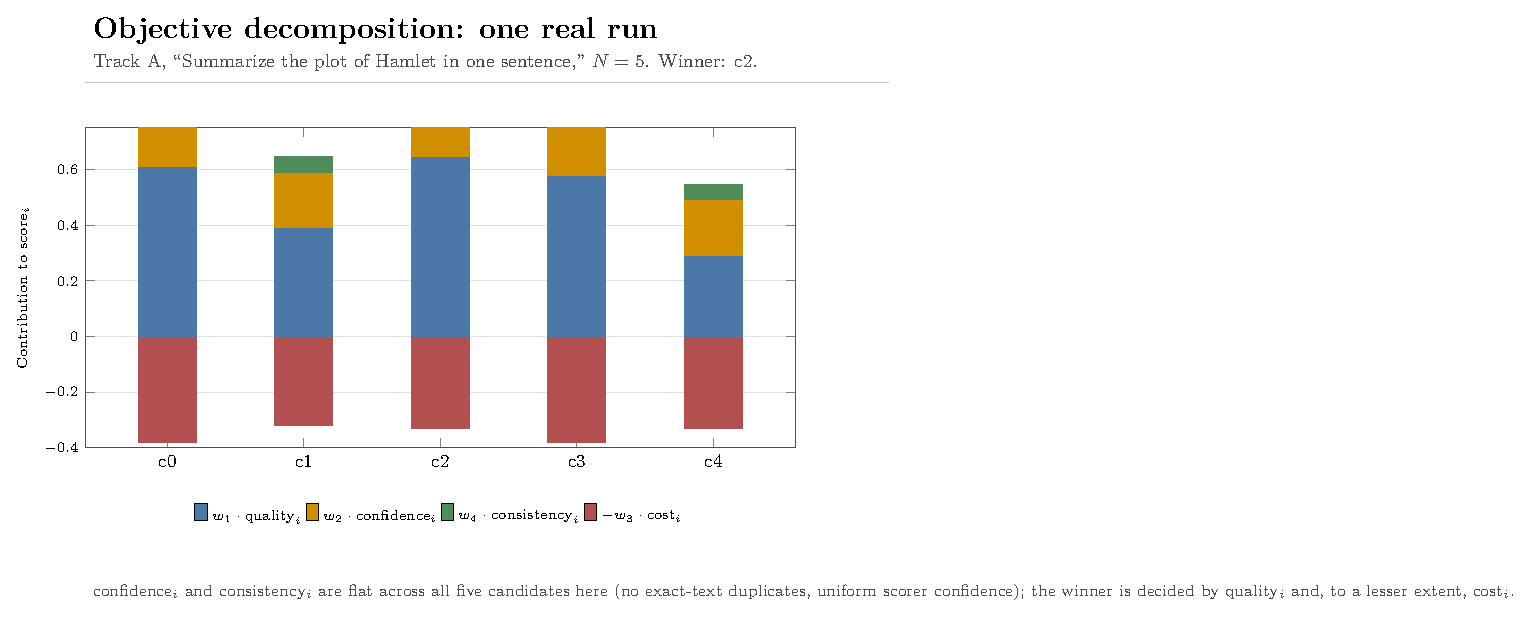
\includegraphics[width=0.85\textwidth]{Figure_3_WorkedExample.pdf}
\caption{The same run as Table~\ref{tab:worked-example}, as stacked weighted
contributions to $\text{score}_i$. Confidence and consistency are constant
across candidates here (no duplicates; uniform scorer confidence), so the
ranking is decided by quality and cost. These candidates are one-sentence
summaries; on multi-hundred-word reasoning outputs the cost term is far
larger relative to quality (Section~\ref{M-sec:cost-diagnosis}).}
\label{fig:worked-example}
\end{figure}


\begin{figure}[htbp]
\centering
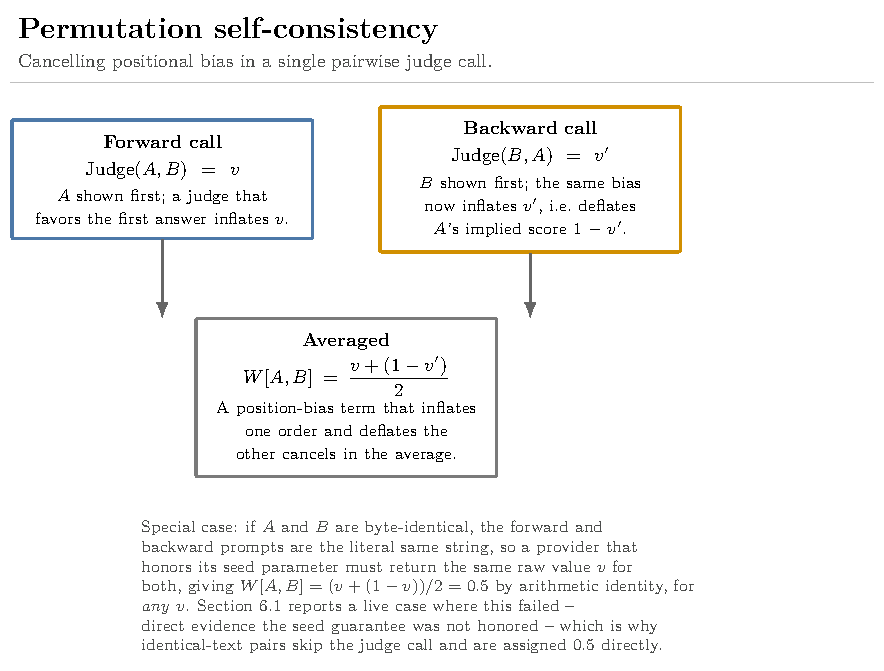
\includegraphics[width=0.85\textwidth]{Figure_2_BiasCancellation.pdf}
\caption{Permutation self-consistency cancels positional bias by averaging
the forward and (complement-transformed) backward judge calls for each
pair. Byte-identical candidates force $W=0.5$ by arithmetic identity,
independent of the judge's output.}
\label{fig:bias-cancel}
\end{figure}



\bibliographystyle{apalike-ejor}
\bibliography{refs}

\end{document}
